\documentclass{standalone}
\usepackage{tikz}
\usetikzlibrary{patterns, positioning}
\usepackage[sfdefault]{ClearSans} %% option 'sfdefault' activates Clear Sans as the default text font
\usepackage[T1]{fontenc}

\begin{document}
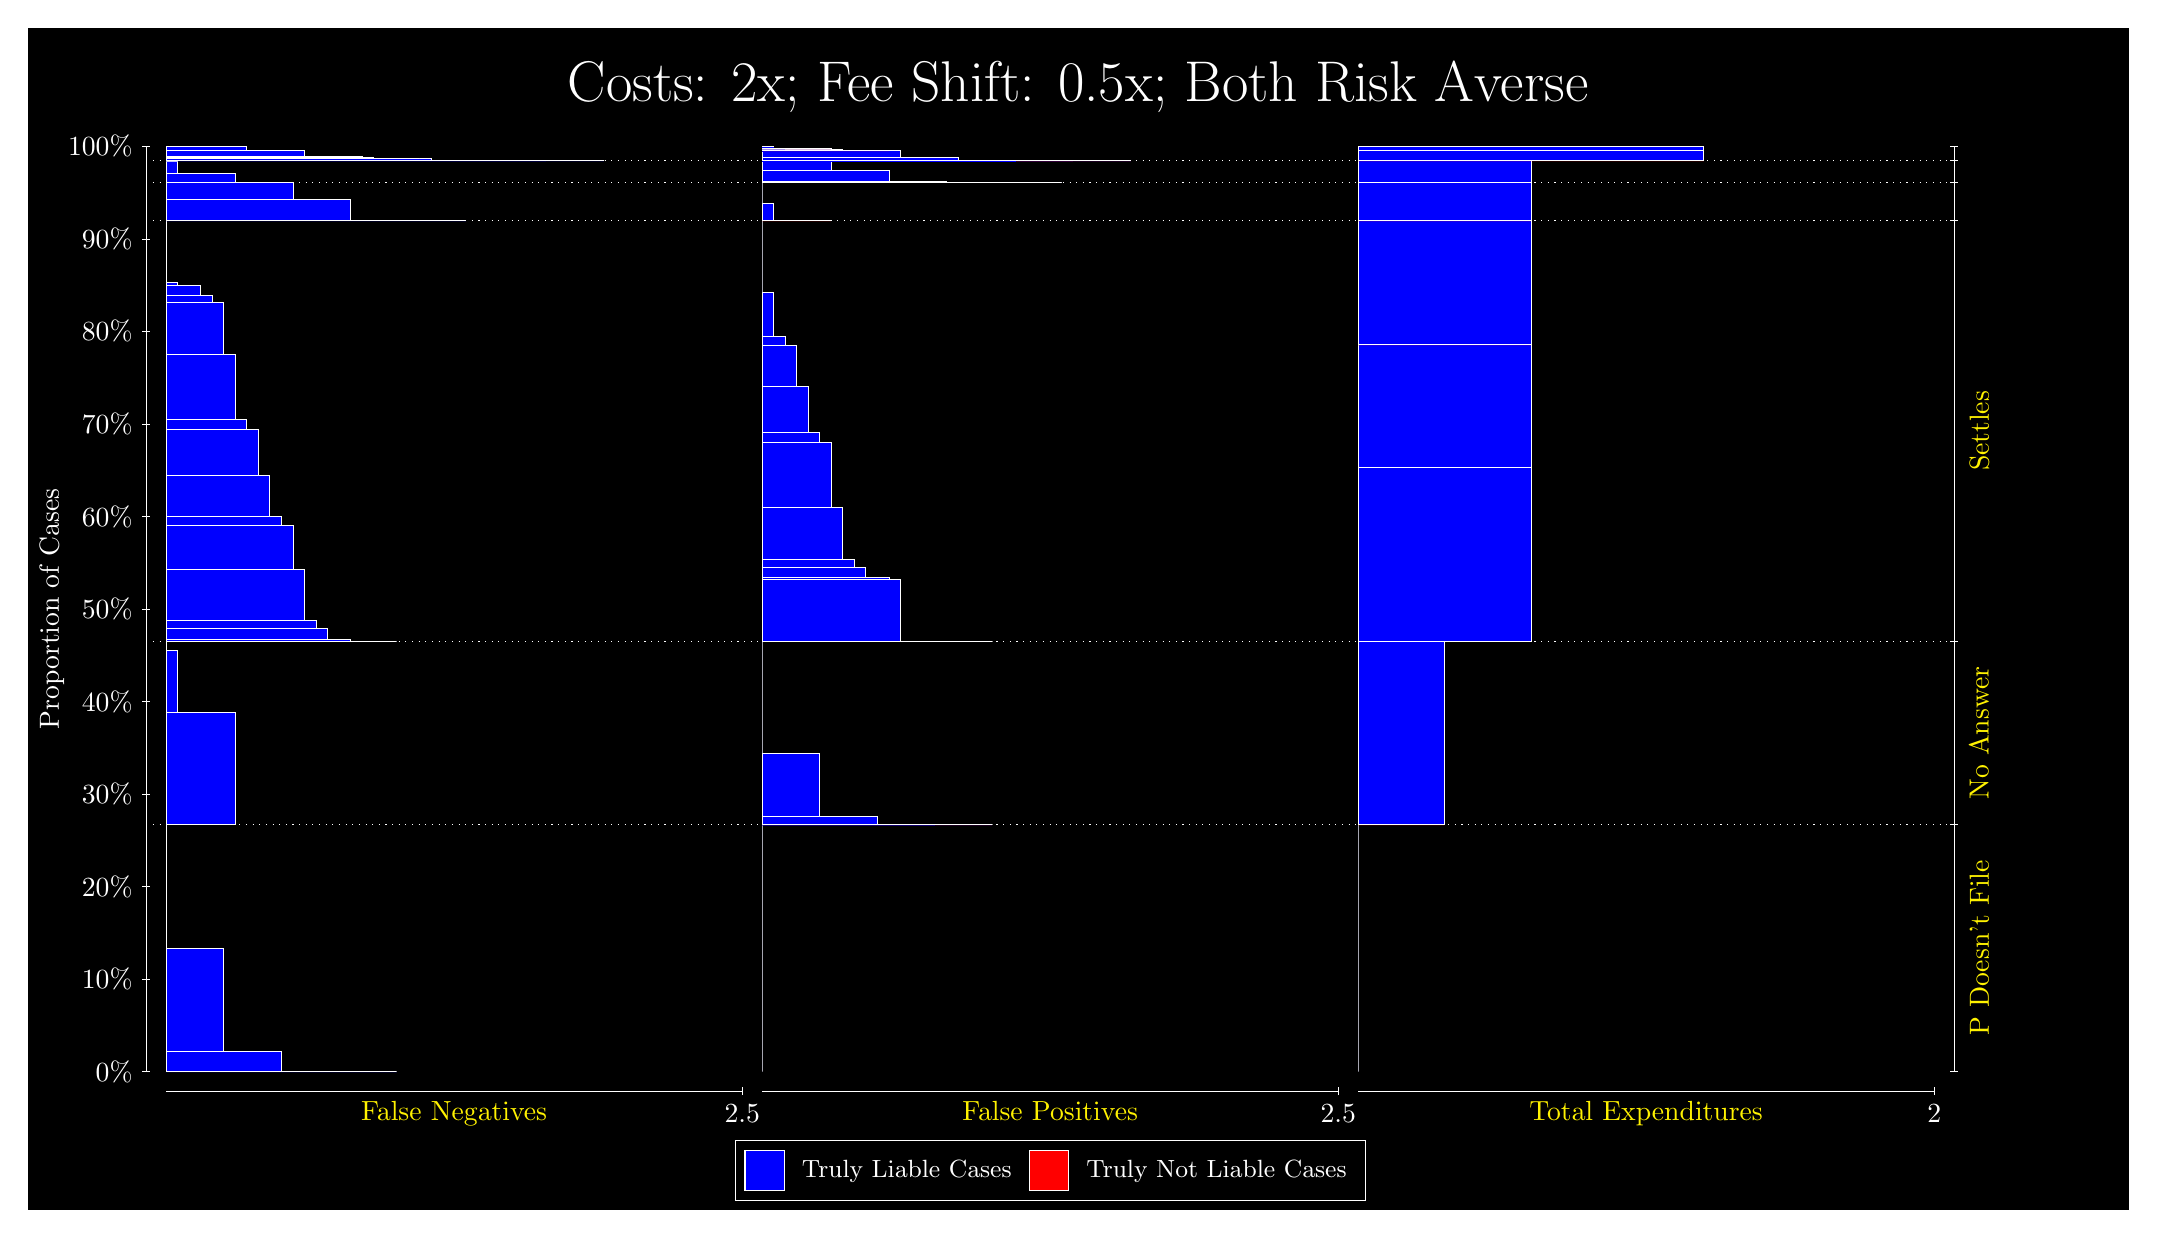
\begin{tikzpicture}
\draw[fill=black] (0,0) rectangle (26.667,15);
\draw[text=white] (0,13.5) rectangle (26.667,15) node[midway] {\huge Costs: 2x; Fee Shift: 0.5x; Both Risk Averse};
\draw[white, very thin] (1.5,1.75) -- (1.5,13.5);
\node[rotate=90, text=white, anchor=center] at (0.3, 7.625) {Proportion of Cases};
\draw[white, very thin] (1.45,1.75) -- (1.55,1.75);
\node[text=white, anchor=east] at (1.45, 1.75) {0\%};
\draw[white, very thin] (1.45,2.925) -- (1.55,2.925);
\node[text=white, anchor=east] at (1.45, 2.925) {10\%};
\draw[white, very thin] (1.45,4.1) -- (1.55,4.1);
\node[text=white, anchor=east] at (1.45, 4.1) {20\%};
\draw[white, very thin] (1.45,5.275) -- (1.55,5.275);
\node[text=white, anchor=east] at (1.45, 5.275) {30\%};
\draw[white, very thin] (1.45,6.45) -- (1.55,6.45);
\node[text=white, anchor=east] at (1.45, 6.45) {40\%};
\draw[white, very thin] (1.45,7.625) -- (1.55,7.625);
\node[text=white, anchor=east] at (1.45, 7.625) {50\%};
\draw[white, very thin] (1.45,8.8) -- (1.55,8.8);
\node[text=white, anchor=east] at (1.45, 8.8) {60\%};
\draw[white, very thin] (1.45,9.975) -- (1.55,9.975);
\node[text=white, anchor=east] at (1.45, 9.975) {70\%};
\draw[white, very thin] (1.45,11.15) -- (1.55,11.15);
\node[text=white, anchor=east] at (1.45, 11.15) {80\%};
\draw[white, very thin] (1.45,12.325) -- (1.55,12.325);
\node[text=white, anchor=east] at (1.45, 12.325) {90\%};
\draw[white, very thin] (1.45,13.5) -- (1.55,13.5);
\node[text=white, anchor=east] at (1.45, 13.5) {100\%};

\draw[white, very thin] (24.457,1.75) -- (24.457,13.5);
\draw[white, very thin] (24.407,1.75) -- (24.507,1.75);
\node[anchor=west] at (24.407, 1.75) {};
\draw[white, very thin] (24.407,4.8857) -- (24.507,4.8857);
\node[anchor=west] at (24.407, 4.8857) {};
\draw[white, very thin] (24.407,7.214) -- (24.507,7.214);
\node[anchor=west] at (24.407, 7.214) {};
\draw[white, very thin] (24.407,12.557) -- (24.507,12.557);
\node[anchor=west] at (24.407, 12.557) {};
\draw[white, very thin] (24.407,13.045) -- (24.507,13.045);
\node[anchor=west] at (24.407, 13.045) {};
\draw[white, very thin] (24.407,13.317) -- (24.507,13.317);
\node[anchor=west] at (24.407, 13.317) {};
\draw[white, very thin] (24.407,13.5) -- (24.507,13.5);
\node[anchor=west] at (24.407, 13.5) {};

\draw[white, very thin, fill=blue] (1.75,1.75) rectangle (4.6775,1.75);
\draw[white, very thin, fill=blue] (1.75,1.75) rectangle (3.9457,1.7526);
\draw[white, very thin, fill=blue] (1.75,1.7526) rectangle (3.2138,2.0033);
\draw[white, very thin, fill=blue] (1.75,2.0033) rectangle (2.4819,3.3215);
\draw[white, very thin, fill=red] (1.75,3.3215) rectangle (1.75,3.3215);
\draw[white, very thin, fill=blue] (1.75,3.3215) rectangle (1.75,4.8857);
\draw[white, very thin, fill=blue] (1.75,4.8857) rectangle (2.6283,6.3076);
\draw[white, very thin, fill=blue] (1.75,6.3076) rectangle (1.8964,7.1045);
\draw[white, very thin, fill=red] (1.75,7.1045) rectangle (1.75,7.1045);
\draw[white, very thin, fill=blue] (1.75,7.1045) rectangle (1.75,7.214);
\draw[white, very thin, fill=blue] (1.75,7.214) rectangle (4.6775,7.214);
\draw[white, very thin, fill=blue] (1.75,7.214) rectangle (4.3848,7.2142);
\draw[white, very thin, fill=blue] (1.75,7.2142) rectangle (4.092,7.2384);
\draw[white, very thin, fill=blue] (1.75,7.2384) rectangle (3.9457,7.2388);
\draw[white, very thin, fill=blue] (1.75,7.2388) rectangle (3.7993,7.3783);
\draw[white, very thin, fill=blue] (1.75,7.3783) rectangle (3.6529,7.4821);
\draw[white, very thin, fill=blue] (1.75,7.4821) rectangle (3.5065,8.1247);
\draw[white, very thin, fill=blue] (1.75,8.1247) rectangle (3.3602,8.687);
\draw[white, very thin, fill=blue] (1.75,8.687) rectangle (3.2138,8.7977);
\draw[white, very thin, fill=blue] (1.75,8.7977) rectangle (3.0674,9.322);
\draw[white, very thin, fill=blue] (1.75,9.322) rectangle (2.921,9.904);
\draw[white, very thin, fill=blue] (1.75,9.904) rectangle (2.7746,10.032);
\draw[white, very thin, fill=blue] (1.75,10.032) rectangle (2.6283,10.856);
\draw[white, very thin, fill=blue] (1.75,10.856) rectangle (2.4819,11.515);
\draw[white, very thin, fill=blue] (1.75,11.515) rectangle (2.3355,11.614);
\draw[white, very thin, fill=blue] (1.75,11.614) rectangle (2.1891,11.74);
\draw[white, very thin, fill=blue] (1.75,11.74) rectangle (2.0428,11.741);
\draw[white, very thin, fill=blue] (1.75,11.741) rectangle (1.8964,11.773);
\draw[white, very thin, fill=red] (1.75,11.773) rectangle (1.75,11.773);
\draw[white, very thin, fill=blue] (1.75,11.773) rectangle (1.75,12.557);
\draw[white, very thin, fill=blue] (1.75,12.557) rectangle (5.5558,12.557);
\draw[white, very thin, fill=blue] (1.75,12.557) rectangle (4.8239,12.563);
\draw[white, very thin, fill=blue] (1.75,12.563) rectangle (4.092,12.831);
\draw[white, very thin, fill=blue] (1.75,12.831) rectangle (3.3602,13.042);
\draw[white, very thin, fill=blue] (1.75,13.042) rectangle (2.6283,13.045);
\draw[white, very thin, fill=red] (1.75,13.045) rectangle (1.75,13.045);
\draw[white, very thin, fill=blue] (1.75,13.045) rectangle (2.6283,13.164);
\draw[white, very thin, fill=blue] (1.75,13.164) rectangle (1.8964,13.31);
\draw[white, very thin, fill=red] (1.75,13.31) rectangle (1.75,13.31);
\draw[white, very thin, fill=blue] (1.75,13.31) rectangle (1.75,13.317);
\draw[white, very thin, fill=blue] (1.75,13.317) rectangle (7.3123,13.317);
\draw[white, very thin, fill=blue] (1.75,13.317) rectangle (6.5805,13.317);
\draw[white, very thin, fill=blue] (1.75,13.317) rectangle (5.8486,13.321);
\draw[white, very thin, fill=blue] (1.75,13.321) rectangle (5.7022,13.321);
\draw[white, very thin, fill=blue] (1.75,13.321) rectangle (5.1167,13.347);
\draw[white, very thin, fill=blue] (1.75,13.347) rectangle (4.9703,13.347);
\draw[white, very thin, fill=blue] (1.75,13.347) rectangle (4.3848,13.355);
\draw[white, very thin, fill=blue] (1.75,13.355) rectangle (4.2384,13.372);
\draw[white, very thin, fill=blue] (1.75,13.372) rectangle (3.6529,13.372);
\draw[white, very thin, fill=blue] (1.75,13.372) rectangle (3.5065,13.456);
\draw[white, very thin, fill=blue] (1.75,13.456) rectangle (2.921,13.456);
\draw[white, very thin, fill=blue] (1.75,13.456) rectangle (2.7746,13.498);
\draw[white, very thin, fill=blue] (1.75,13.498) rectangle (2.0428,13.5);
\draw[white, very thin, fill=red] (1.75,13.5) rectangle (1.75,13.5);
\draw[white, very thin, fill=blue] (1.75,13.5) rectangle (1.75,13.5);
\draw[white, very thin, fill=red] (9.3189,1.75) rectangle (9.3189,1.75);
\draw[white, very thin, fill=blue] (9.3189,1.75) rectangle (9.3189,4.8857);
\draw[white, very thin, fill=red] (9.3189,4.8857) rectangle (12.246,4.8857);
\draw[white, very thin, fill=blue] (9.3189,4.8857) rectangle (12.246,4.8857);
\draw[white, very thin, fill=blue] (9.3189,4.8857) rectangle (11.515,4.8859);
\draw[white, very thin, fill=blue] (9.3189,4.8859) rectangle (10.783,4.9951);
\draw[white, very thin, fill=blue] (9.3189,4.9951) rectangle (10.051,5.792);
\draw[white, very thin, fill=blue] (9.3189,5.792) rectangle (9.3189,7.214);
\draw[white, very thin, fill=red] (9.3189,7.214) rectangle (12.246,7.214);
\draw[white, very thin, fill=blue] (9.3189,7.214) rectangle (12.246,7.214);
\draw[white, very thin, fill=red] (9.3189,7.214) rectangle (11.954,7.214);
\draw[white, very thin, fill=blue] (9.3189,7.214) rectangle (11.954,7.214);
\draw[white, very thin, fill=red] (9.3189,7.214) rectangle (11.661,7.214);
\draw[white, very thin, fill=blue] (9.3189,7.214) rectangle (11.661,7.214);
\draw[white, very thin, fill=blue] (9.3189,7.214) rectangle (11.515,7.214);
\draw[white, very thin, fill=red] (9.3189,7.214) rectangle (11.368,7.214);
\draw[white, very thin, fill=blue] (9.3189,7.214) rectangle (11.368,7.2152);
\draw[white, very thin, fill=blue] (9.3189,7.2152) rectangle (11.222,7.2154);
\draw[white, very thin, fill=red] (9.3189,7.2154) rectangle (11.075,7.2154);
\draw[white, very thin, fill=blue] (9.3189,7.2154) rectangle (11.075,7.9975);
\draw[white, very thin, fill=blue] (9.3189,7.9975) rectangle (10.929,8.0294);
\draw[white, very thin, fill=blue] (9.3189,8.0294) rectangle (10.783,8.0307);
\draw[white, very thin, fill=blue] (9.3189,8.0307) rectangle (10.636,8.1566);
\draw[white, very thin, fill=blue] (9.3189,8.1566) rectangle (10.49,8.2555);
\draw[white, very thin, fill=blue] (9.3189,8.2555) rectangle (10.344,8.9147);
\draw[white, very thin, fill=blue] (9.3189,8.9147) rectangle (10.197,9.7386);
\draw[white, very thin, fill=blue] (9.3189,9.7386) rectangle (10.051,9.8669);
\draw[white, very thin, fill=blue] (9.3189,9.8669) rectangle (9.9044,10.449);
\draw[white, very thin, fill=blue] (9.3189,10.449) rectangle (9.758,10.973);
\draw[white, very thin, fill=blue] (9.3189,10.973) rectangle (9.6116,11.084);
\draw[white, very thin, fill=blue] (9.3189,11.084) rectangle (9.4652,11.646);
\draw[white, very thin, fill=blue] (9.3189,11.646) rectangle (9.3189,12.557);
\draw[white, very thin, fill=red] (9.3189,12.557) rectangle (10.197,12.557);
\draw[white, very thin, fill=blue] (9.3189,12.557) rectangle (10.197,12.559);
\draw[white, very thin, fill=blue] (9.3189,12.559) rectangle (9.4652,12.771);
\draw[white, very thin, fill=blue] (9.3189,12.771) rectangle (9.3189,13.045);
\draw[white, very thin, fill=red] (9.3189,13.045) rectangle (13.125,13.045);
\draw[white, very thin, fill=blue] (9.3189,13.045) rectangle (13.125,13.045);
\draw[white, very thin, fill=blue] (9.3189,13.045) rectangle (12.393,13.045);
\draw[white, very thin, fill=blue] (9.3189,13.045) rectangle (11.661,13.052);
\draw[white, very thin, fill=blue] (9.3189,13.052) rectangle (10.929,13.198);
\draw[white, very thin, fill=blue] (9.3189,13.198) rectangle (10.197,13.317);
\draw[white, very thin, fill=red] (9.3189,13.317) rectangle (14.003,13.317);
\draw[white, very thin, fill=blue] (9.3189,13.317) rectangle (14.003,13.317);
\draw[white, very thin, fill=red] (9.3189,13.317) rectangle (13.271,13.317);
\draw[white, very thin, fill=blue] (9.3189,13.317) rectangle (13.271,13.317);
\draw[white, very thin, fill=red] (9.3189,13.317) rectangle (12.539,13.317);
\draw[white, very thin, fill=blue] (9.3189,13.317) rectangle (12.539,13.319);
\draw[white, very thin, fill=blue] (9.3189,13.319) rectangle (11.807,13.361);
\draw[white, very thin, fill=red] (9.3189,13.361) rectangle (11.807,13.361);
\draw[white, very thin, fill=blue] (9.3189,13.361) rectangle (11.807,13.361);
\draw[white, very thin, fill=red] (9.3189,13.361) rectangle (11.661,13.361);
\draw[white, very thin, fill=blue] (9.3189,13.361) rectangle (11.661,13.361);
\draw[white, very thin, fill=blue] (9.3189,13.361) rectangle (11.075,13.445);
\draw[white, very thin, fill=blue] (9.3189,13.445) rectangle (11.075,13.446);
\draw[white, very thin, fill=red] (9.3189,13.446) rectangle (10.929,13.446);
\draw[white, very thin, fill=blue] (9.3189,13.446) rectangle (10.929,13.446);
\draw[white, very thin, fill=blue] (9.3189,13.446) rectangle (10.344,13.454);
\draw[white, very thin, fill=blue] (9.3189,13.454) rectangle (10.344,13.462);
\draw[white, very thin, fill=blue] (9.3189,13.462) rectangle (10.197,13.47);
\draw[white, very thin, fill=red] (9.3189,13.47) rectangle (10.197,13.47);
\draw[white, very thin, fill=blue] (9.3189,13.47) rectangle (10.197,13.47);
\draw[white, very thin, fill=blue] (9.3189,13.47) rectangle (9.6116,13.47);
\draw[white, very thin, fill=blue] (9.3189,13.47) rectangle (9.6116,13.47);
\draw[white, very thin, fill=blue] (9.3189,13.47) rectangle (9.4652,13.495);
\draw[white, very thin, fill=blue] (9.3189,13.495) rectangle (9.4652,13.496);
\draw[white, very thin, fill=blue] (9.3189,13.496) rectangle (9.3189,13.5);
\draw[white, very thin, fill=red] (16.888,1.75) rectangle (16.888,1.75);
\draw[white, very thin, fill=blue] (16.888,1.75) rectangle (16.888,4.8857);
\draw[white, very thin, fill=red] (16.888,4.8857) rectangle (17.986,4.8857);
\draw[white, very thin, fill=blue] (16.888,4.8857) rectangle (17.986,7.214);
\draw[white, very thin, fill=red] (16.888,7.214) rectangle (19.083,7.214);
\draw[white, very thin, fill=blue] (16.888,7.214) rectangle (19.083,9.4284);
\draw[white, very thin, fill=red] (16.888,9.4284) rectangle (19.083,9.4284);
\draw[white, very thin, fill=blue] (16.888,9.4284) rectangle (19.083,10.981);
\draw[white, very thin, fill=red] (16.888,10.981) rectangle (19.083,10.981);
\draw[white, very thin, fill=blue] (16.888,10.981) rectangle (19.083,12.557);
\draw[white, very thin, fill=red] (16.888,12.557) rectangle (19.083,12.557);
\draw[white, very thin, fill=blue] (16.888,12.557) rectangle (19.083,13.045);
\draw[white, very thin, fill=red] (16.888,13.045) rectangle (19.083,13.045);
\draw[white, very thin, fill=blue] (16.888,13.045) rectangle (19.083,13.317);
\draw[white, very thin, fill=red] (16.888,13.317) rectangle (21.279,13.317);
\draw[white, very thin, fill=blue] (16.888,13.317) rectangle (21.279,13.453);
\draw[white, very thin, fill=red] (16.888,13.453) rectangle (21.279,13.453);
\draw[white, very thin, fill=blue] (16.888,13.453) rectangle (21.279,13.5);
\draw[white, dotted] (1.5,4.8857) -- (24.457,4.8857);
\draw[white, dotted] (1.5,7.214) -- (24.457,7.214);
\draw[white, dotted] (1.5,12.557) -- (24.457,12.557);
\draw[white, dotted] (1.5,13.045) -- (24.457,13.045);
\draw[white, dotted] (1.5,13.317) -- (24.457,13.317);
\draw[white, very thin] (1.75,1.5) -- (9.0689,1.5);
\node[text=yellow, anchor=north] at (5.4094, 1.5) {False Negatives};
\draw[white, very thin] (9.0689,1.45) -- (9.0689,1.55);
\node[text=white, anchor=north] at (9.0689, 1.45) {2.5};

\draw[white, very thin] (9.3189,1.5) -- (16.638,1.5);
\node[text=yellow, anchor=north] at (12.978, 1.5) {False Positives};
\draw[white, very thin] (16.638,1.45) -- (16.638,1.55);
\node[text=white, anchor=north] at (16.638, 1.45) {2.5};

\draw[white, very thin] (16.888,1.5) -- (24.207,1.5);
\node[text=yellow, anchor=north] at (20.547, 1.5) {Total Expenditures};
\draw[white, very thin] (24.207,1.45) -- (24.207,1.55);
\node[text=white, anchor=north] at (24.207, 1.45) {2};

\node[text=yellow, centered, rotate=90] at (24.777, 3.3178) {P Doesn't File};
\node[text=yellow, centered, rotate=90] at (24.777, 6.0498) {No Answer};
\node[text=yellow, centered, rotate=90] at (24.777, 9.8855) {Settles};




\draw (12.978300999999998,1.5) node[draw=none] (baseCoordinate) {};
\begin{scope}[align=center]
        \matrix[scale=0.5, draw=white, below=0.5cm of baseCoordinate, nodes={draw}, column sep=0.1cm]{
            \node[rectangle, draw, minimum width=0.5cm, minimum height=0.5cm, fill=blue] {}; &
            \node[draw=none, font=\small, text=white] (B) {Truly Liable Cases}; &
            \node[rectangle, draw, minimum width=0.5cm, minimum height=0.5cm, fill=red] {}; &
            \node[draw=none, font=\small, text=white] (B) {Truly Not Liable Cases}; \\
            };
\end{scope}

\end{tikzpicture}
\end{document}